 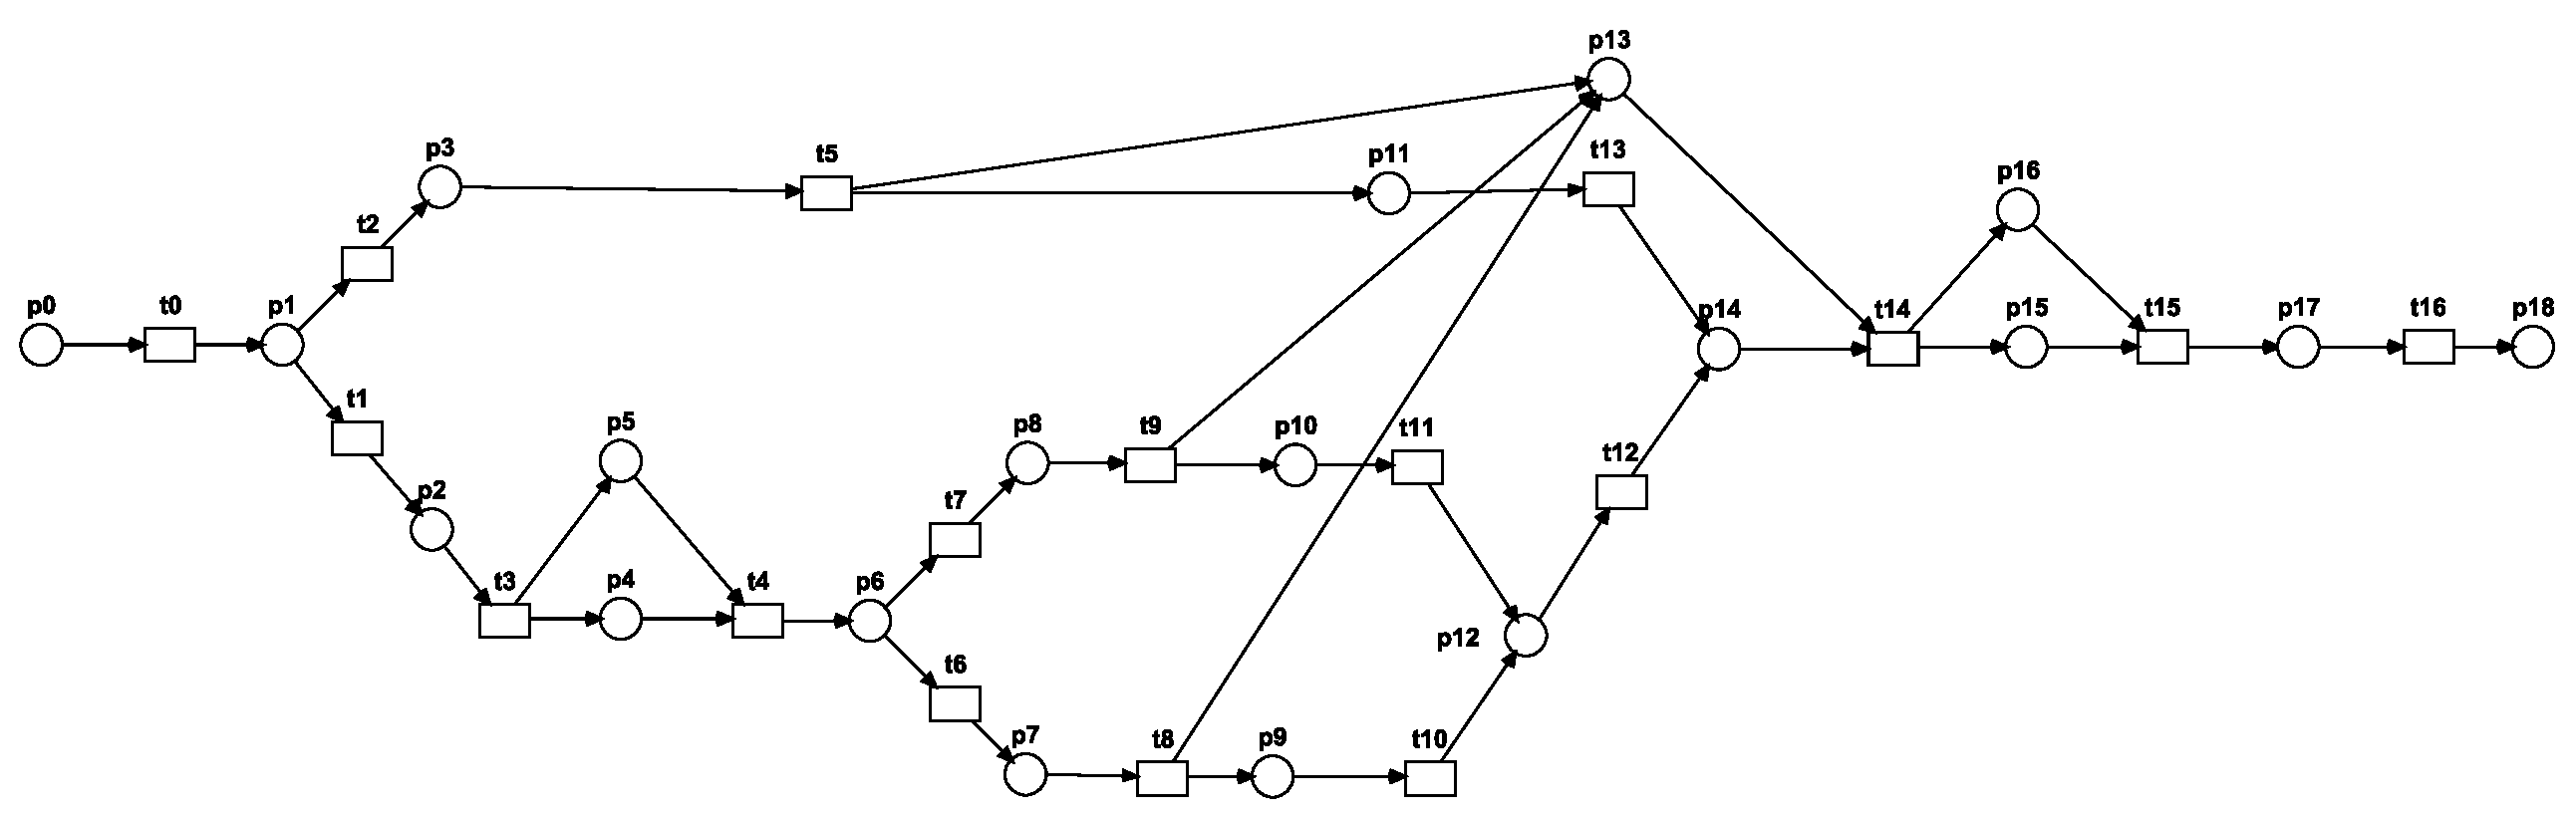
\includegraphics[scale=0.3]{Teilaufgaben/vorlage.pdf}\\
 Anwenden d	er Regel T-Seq:\\
 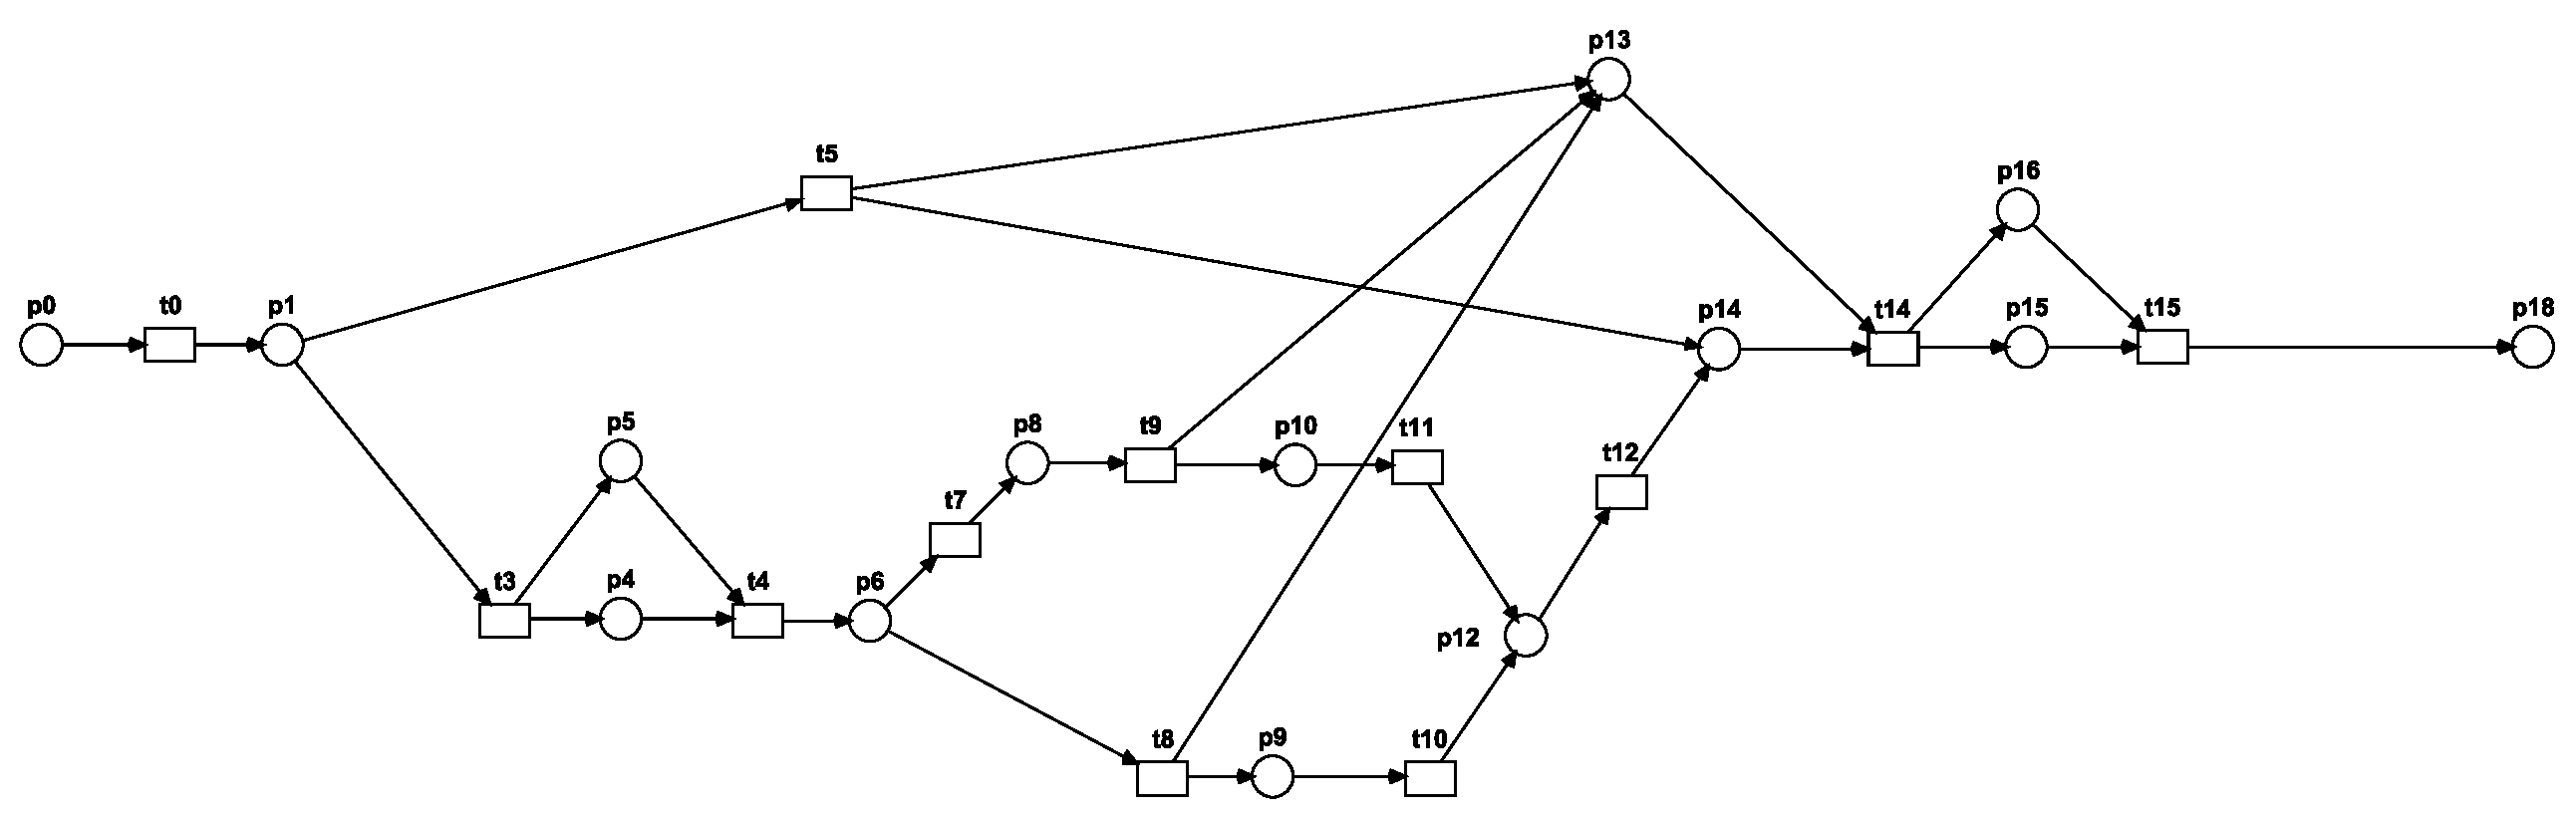
\includegraphics[scale=0.3]{Teilaufgaben/tseq1.pdf}\\
 
  Anwenden der Regel Par:\\
 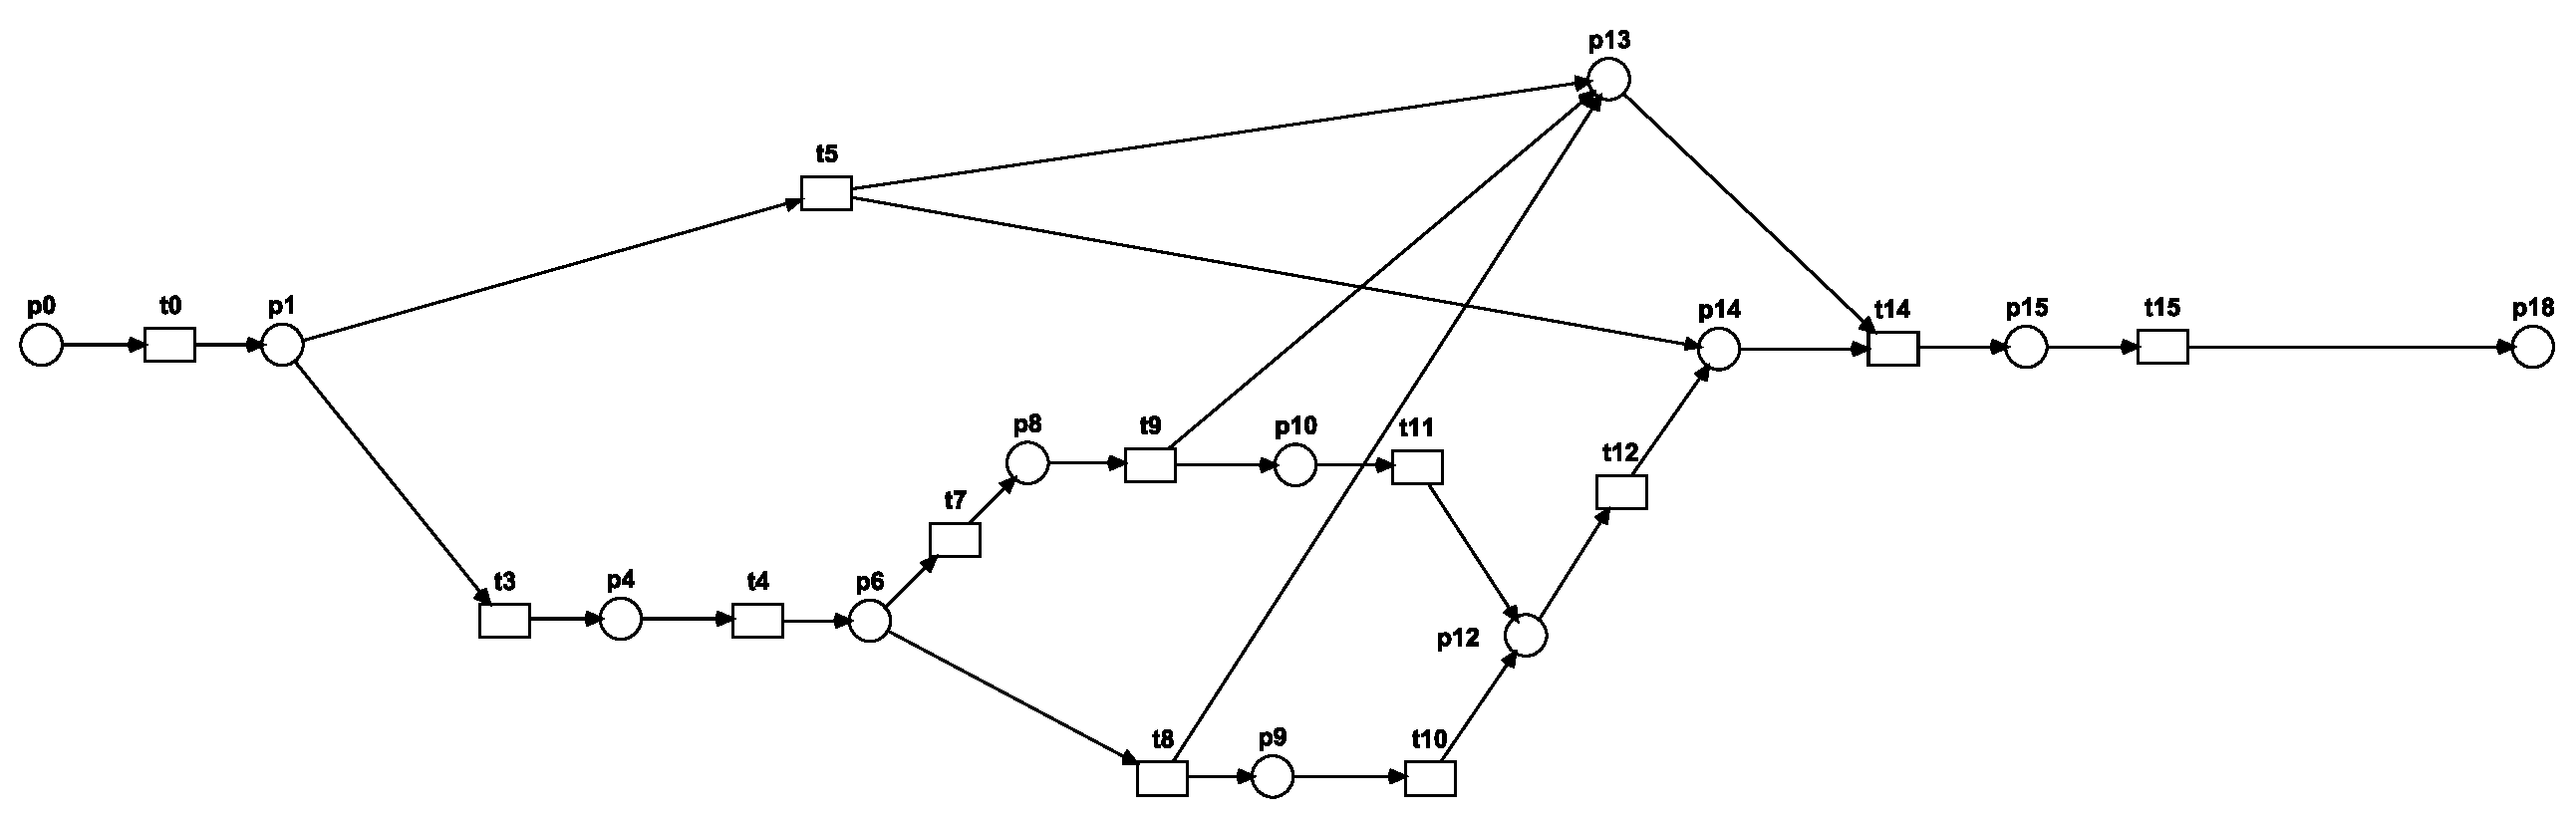
\includegraphics[scale=0.3]{Teilaufgaben/par1.pdf}\\
 
   Anwenden der Regel P-Seq:\\
 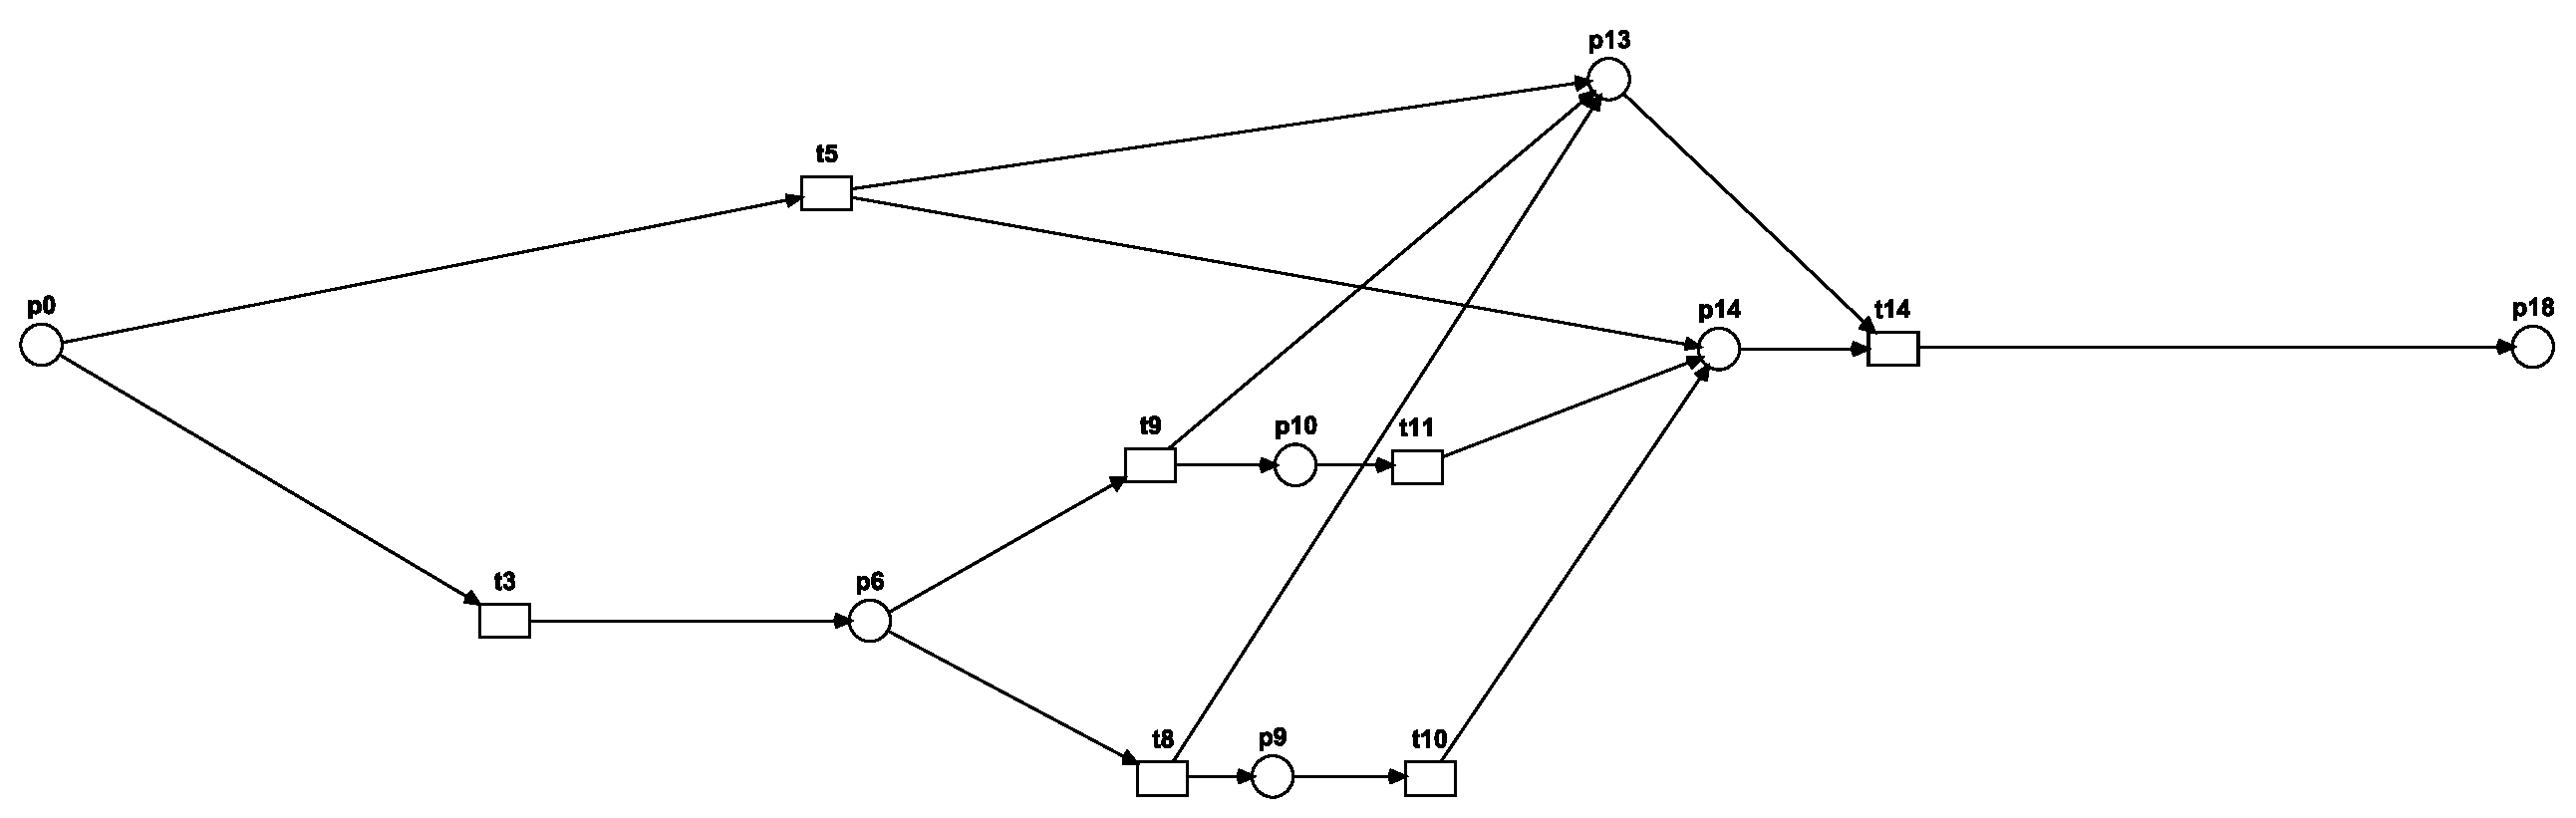
\includegraphics[scale=0.3]{Teilaufgaben/pseq1.pdf}\\
 
    Anwenden der Regel P-Seq:\\
 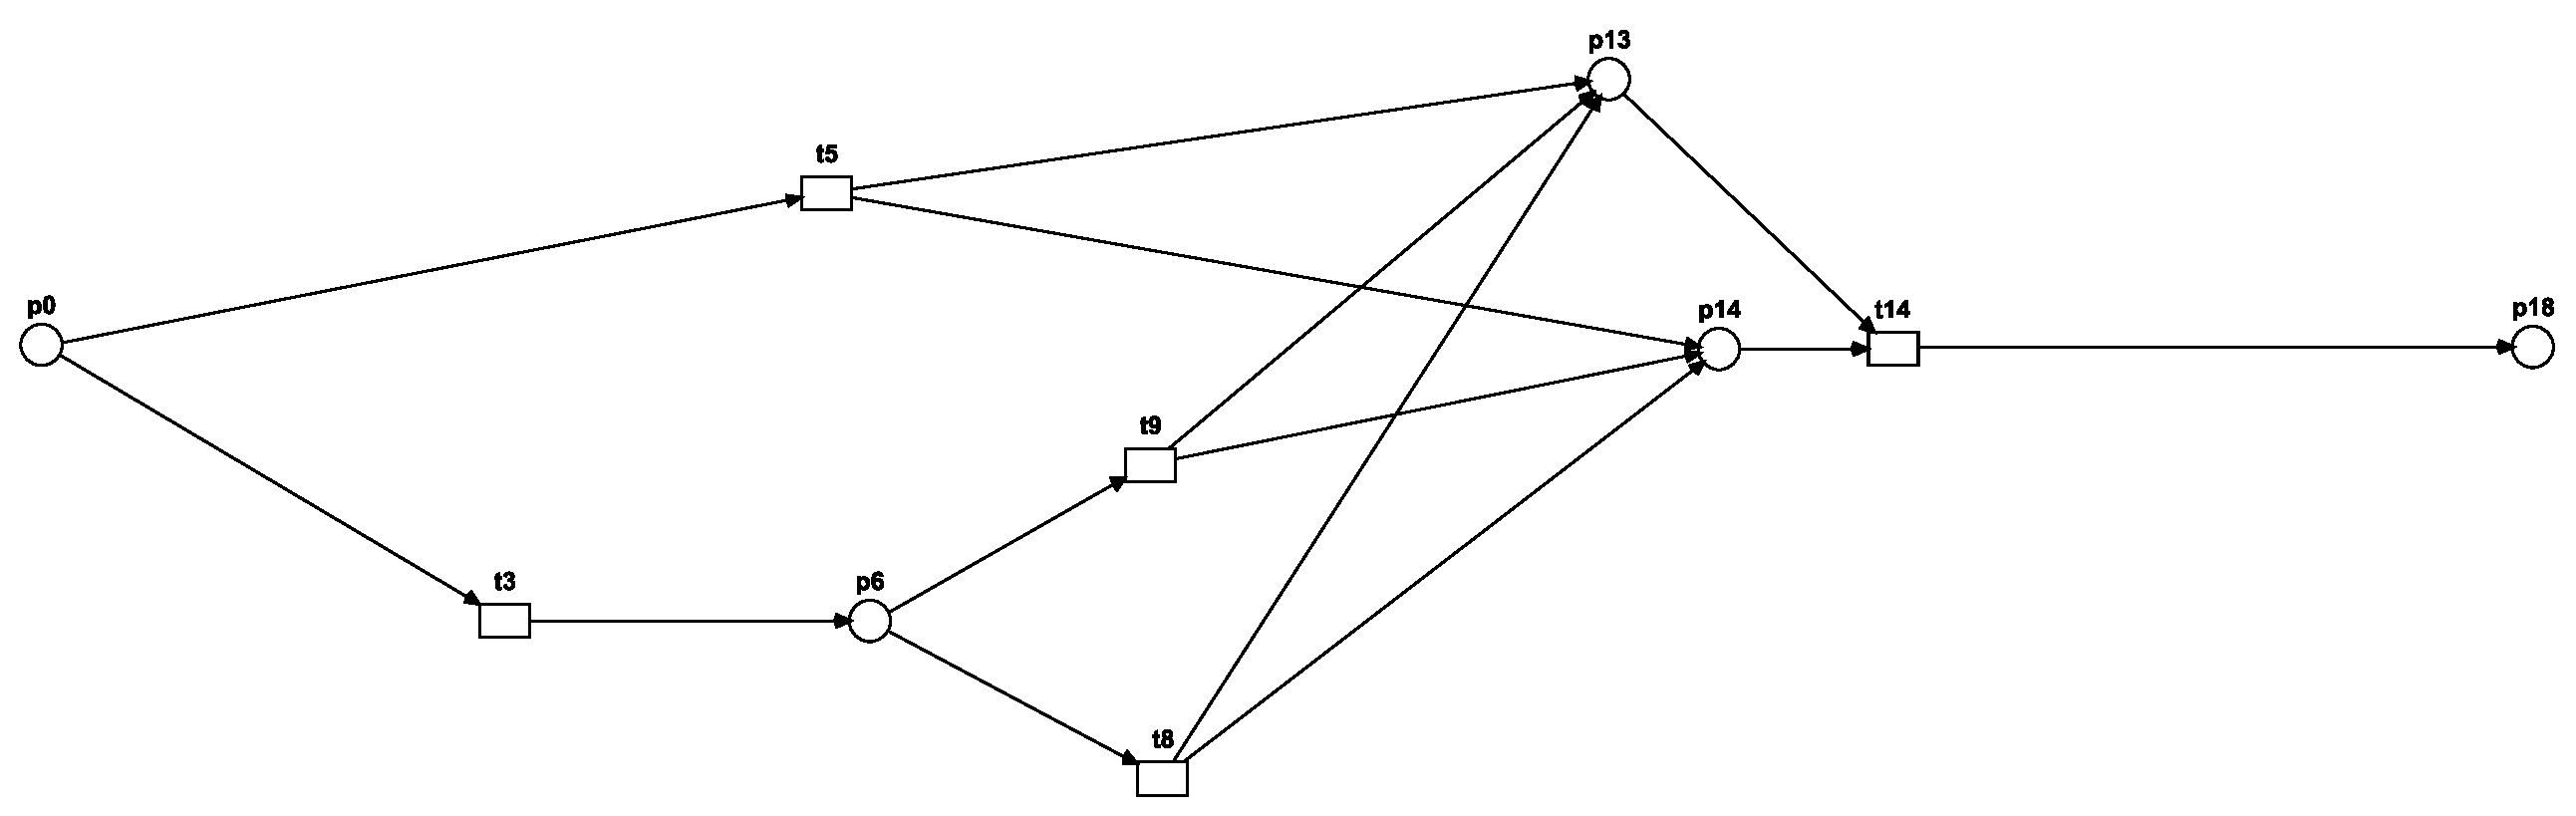
\includegraphics[scale=0.3]{Teilaufgaben/pseq2.pdf}\\
 
     Anwenden der Regel Par:\\
 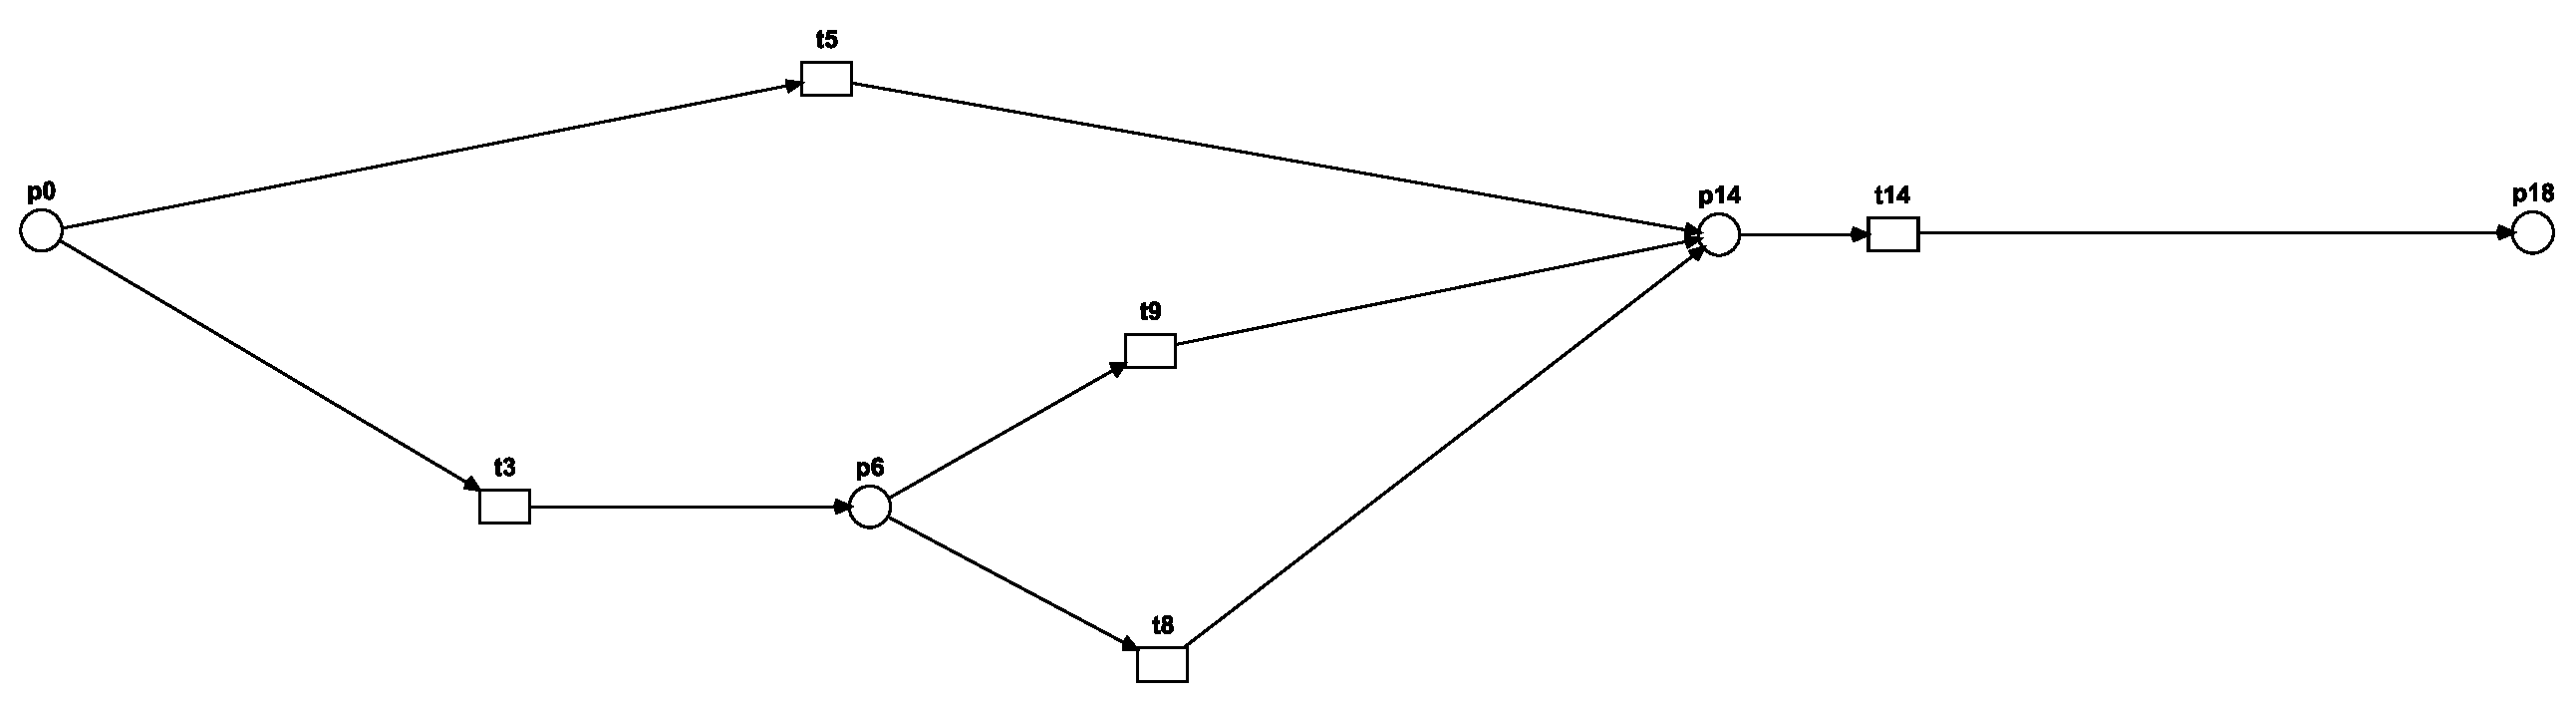
\includegraphics[scale=0.3]{Teilaufgaben/par2.pdf}\\
 
     Anwenden der Regel P-Seq:\\
 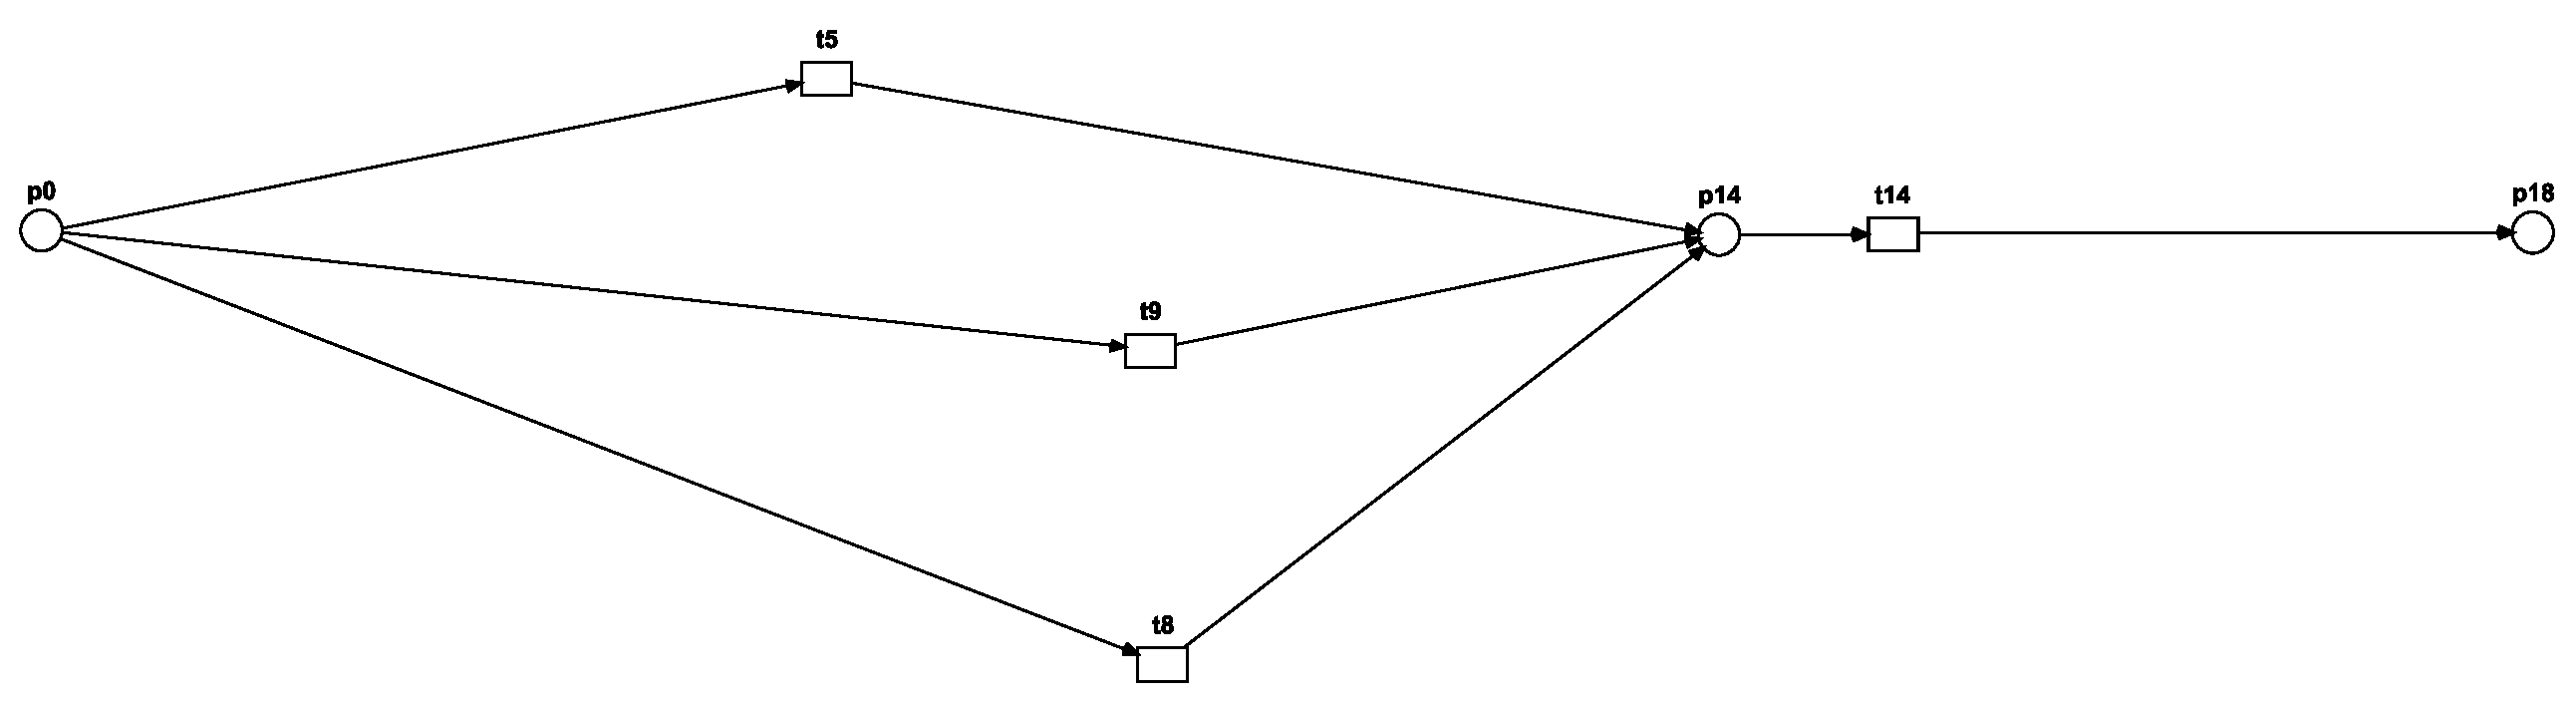
\includegraphics[scale=0.3]{Teilaufgaben/pseq3.pdf}\\
 
      Anwenden der Regel Alt:\\
 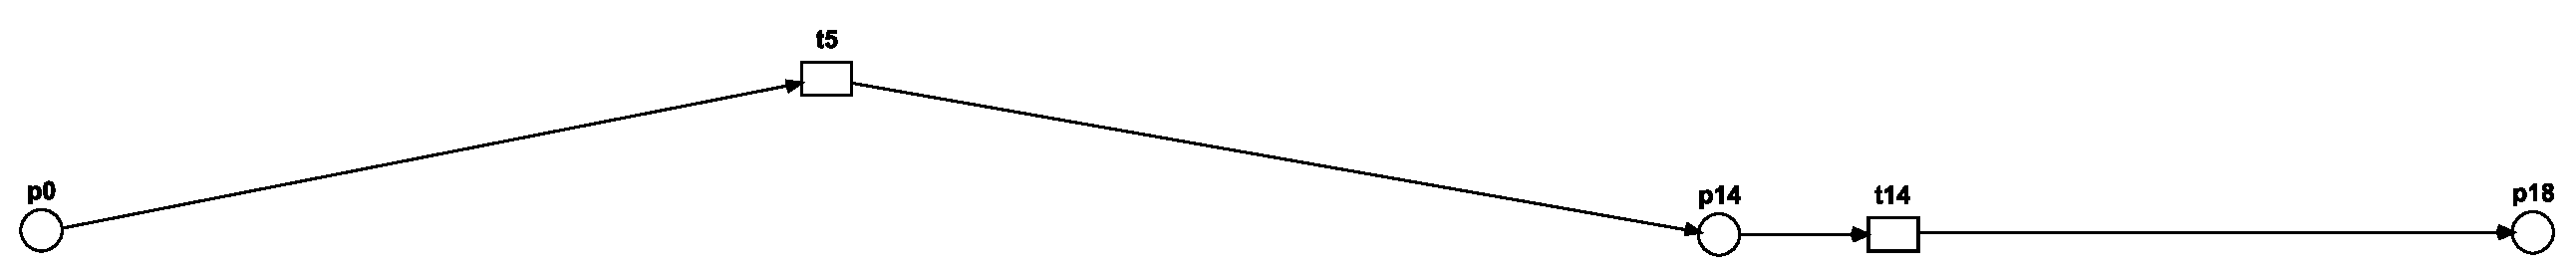
\includegraphics[scale=0.3]{Teilaufgaben/alt1.pdf}\\
 
       Anwenden der Regel T-Seq:\\
 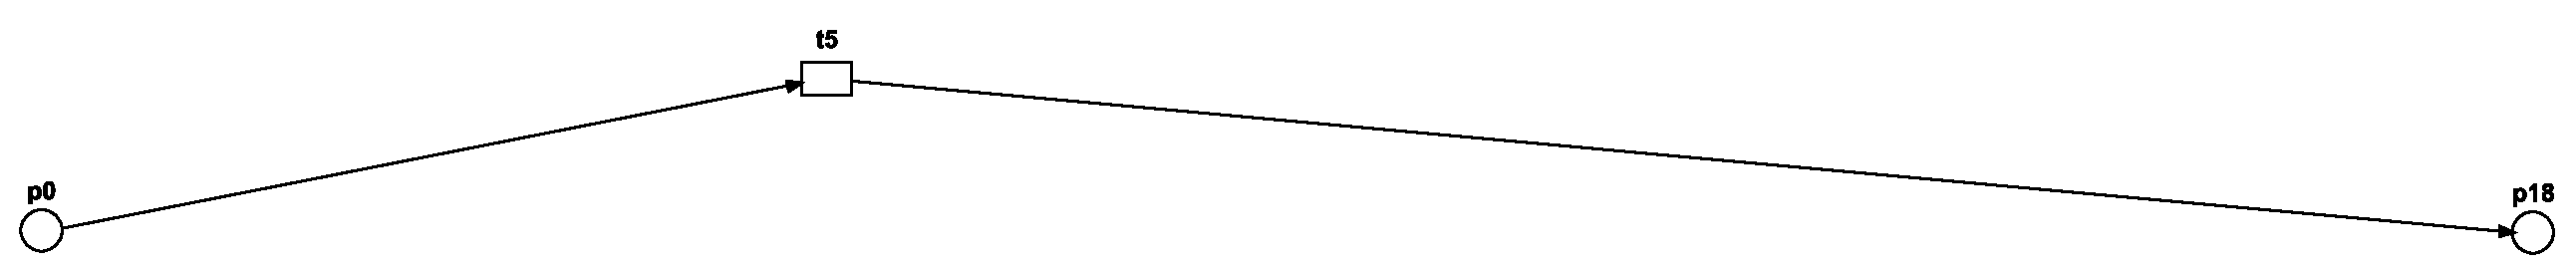
\includegraphics[scale=0.3]{Teilaufgaben/tseq2.pdf}\\
 
 Angekommen Beim trivialen Korrekten Netz, Das Ursprünglihce Netz muss daher auch Korrekt sein.